
\section{Opciones americanas}

Aquellas que pueden ejercerse en cualquier momento antes de su vencimiento. Sea $\Phi(S)$ el payoff de la opción, entonces se cumple que:
\[
\boxed{V \geq \Phi(S)}
\]\label{eq:cond_op_americana}
Si no fuese el caso, entonces $V < \Phi(S) \Rightarrow \Phi(S) - V > 0$, por lo que se podría comprar una opción y ejercer al momento obteniendo un beneficio sin riesgo, por lo que habría arbitraje.

En general, el punto óptimo de ejercicio es aquel que hace que la pendiente de la opción sea la misma que la pendiente del \textit{payoff}.

Sea la cartera
\[
\Pi = V - \Delta S
\]
entonces la diferencia entre el cambio de valor de la cartera y su crecimiento por el interés es:
\[
d\Pi - r\Pi dt = \left( \frac{\partial V}{\partial t} + \frac{1}{2} \sigma^2 S^2 \frac{\partial^2 V}{\partial S^2} - r(V - \Delta S) \right) dt + \left( \frac{\partial V}{\partial S} - \Delta \right) dS
\]
y eligiendo $\Delta = \frac{\partial V}{\partial S}$, se obtiene:
\[
d\Pi - r\Pi dt = \left( \frac{\partial V}{\partial t} + \frac{1}{2} \sigma^2 S^2 \frac{\partial^2 V}{\partial S^2} - rV \right) dt
\]
Para evitar arbitraje solo se debe asegurar que esta resta sea no positiva, de manera que la cartera no gane mas que el interés:
\[
\boxed{\frac{\partial V}{\partial t} + \frac{1}{2} \sigma^2 S^2 \frac{\partial^2 V}{\partial S^2} - rV \leq 0}
\]
El caso $\cdots < 0$ no produce arbitraje porque al vender una opción y meterlo en el banco (para que crezca a ritmo $r$), se corre el riesgo de que el comprador ejerza en cualquier momento.


\subsection{Dividendos discretos}
Como se ha visto en la ecuacion~\eqref{eq:divs_discretos}, si hay dividendo discreto se cumple que $V(S, t_i^-) = V(S - D_i, t_i^+)$, por lo que para evitar que el valor de la opción caiga por debajo del valor de ejercicio inmediato se impone
\[
\boxed{V(S, t_d^-) = \max\left(V(S - D, t_d^+), \Phi(S)\right)}
\]
garantizando que el valor de la opción nunca sea menor que el payoff si se ejerciera justo antes del dividendo evitando así arbitraje.





\subsection{Opciones one-touch}
Es una versión americana de la opción binaria  europea. Se paga una cantidad fija si el subyacente alcanza una cierta barrera antes de vencimiento. El pago realiza tan pronto como se alcanza la barrera, sin esperar al vencimiento.
\begin{itemize}
    \item \textbf{One-touch call:} paga si el subyacente $S$ alcanza un nivel superior $S_u$.
    \[
        \boxed{V(S, t) = \left( \frac{S_u}{S} \right)^{2r/\sigma^2} N(d_6) + \frac{S}{S_u} N(d_1)}
    \]
    donde
    \[
        \boxed{d_6 = \frac{\log(S/S_u) - (r + \frac{1}{2}\sigma^2)(T-t)}{\sigma\sqrt{T-t}}}
    \]
    y $d_1$ es el mismo que en Black-Scholes~\eqref{eq:d_sol_BS}.
    \begin{figure}[H]
        \centering
        \begin{subfigure}[b]{0.35\linewidth}
            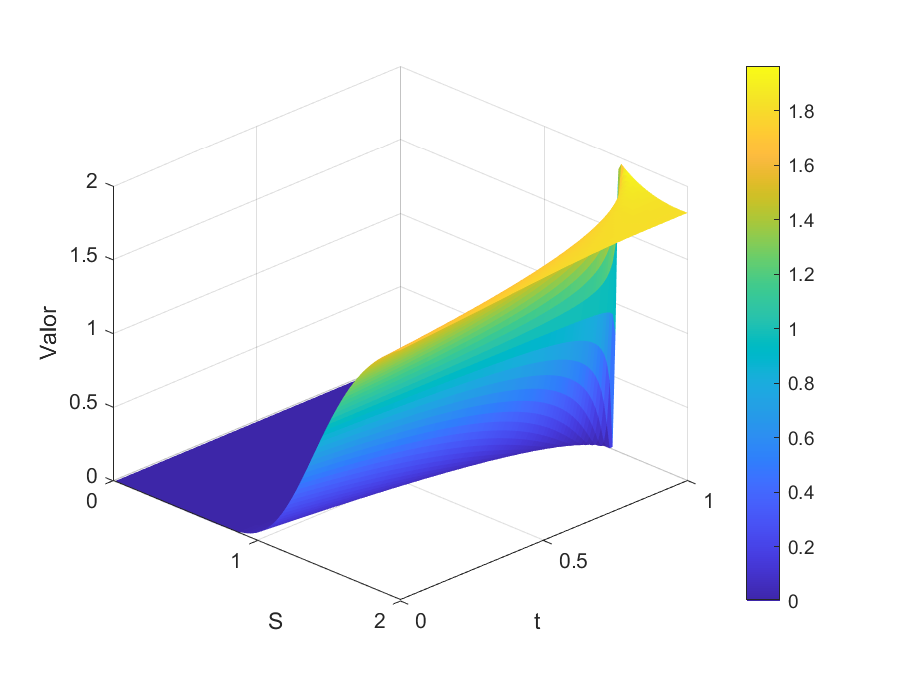
\includegraphics[width=\linewidth]{Imagenes/9_Americanas/One_Touch_Call.eps}
            \caption{Solución de una opción one-touch call}
        \end{subfigure}
        \begin{subfigure}[b]{0.35\linewidth}
            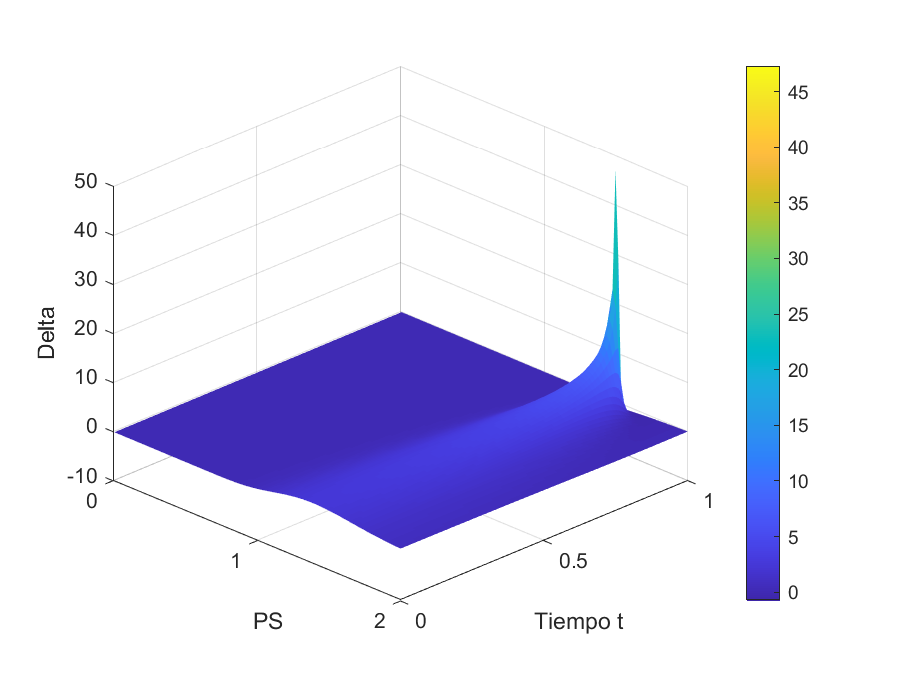
\includegraphics[width=\linewidth]{Imagenes/9_Americanas/Delta_One_Touch_Call.eps}
            \caption{Delta de una opción one-touch call}
        \end{subfigure}
    \end{figure}
    \item \textbf{One-touch put:} paga si $S$ cae hasta un nivel inferior $S_l$.
    \[
        \boxed{V(S, t) = \left( \frac{S_l}{S} \right)^{2r/\sigma^2} N(-d_6) + \frac{S}{S_l} N(-d_1)}
    \]
    con
    \[
        \boxed{d_6 = \frac{\log(S/S_l) - (r + \frac{1}{2}\sigma^2)(T-t)}{\sigma\sqrt{T-t}}}
    \]
    y $d_1$ es el mismo que en Black-Scholes~\eqref{eq:d_sol_BS}.
    \item \textbf{Double one-touch:} paga si $S$ alcanza cualquiera de dos barreras (superior $S_u$ o inferior $S_l$) antes del vencimiento. El valor se puede calcular mediante series de Fourier y no es simplemente la suma de una call y una put one-touch.
\end{itemize}




\subsection{Otros tipos de opciones americanas}
\begin{itemize}
    \item \textbf{Opciones israelíes}: opciones americanas en las que el escritor puede cancelar la opción más temprano pagando una penalización.
    \item \textbf{Opciones Bermuda}: opciones americanas que solo pueden ejercerse en fechas específicas, no en cualquier momento. Lo único que cambia con respecto a las americanas es que la condición~\eqref{eq:cond_op_americana} se aplica solo en los momentos de ejercicio permitido.
    \item \textbf{Opciones Make Your Mind Up}: opciones americanas en las que hay que avisar con cierta antelación si se va a ejercer. Hay más información en el apéndice~\ref{Make_Your_Mind_Up_Instalment}.
    \item \textbf{Opciones instalment}: no son exactamente americanas, pero son similares. Hay más información en el apéndice~\ref{Make_Your_Mind_Up_Instalment}.
\end{itemize}









